\subsection{Three.js}

With the introduction of HTML5, experimentation with the new \texttt{canvas} began. The \texttt{canvas} tag introduces a high performance dynamic scriptable shape rendering capability, which is very useful if doing high-quality 3D graphics or performing super fast animations on the Web without the use of plug-ins \cite{wiki:webgl}. Consequently, large number of projects being built on top of this tag started appearing. One of these projects is the 3D Javascript engine, developed by Ricardo Cabello (a.k.a., MrDoob), called Three.js.  

Three.js engine's functionality provides you with an out-of-the-box WebGL renderer, called WebGLRenderer, and a controllable camera and viewport components. The physics and animation work is up to the developer to work out. Nevertheless, it is not complicated to add up this functionality to Three.js as it is shown in many Three.js examples found online at \cite{threeJS}. Figure~\ref{fig:threejs} illustrates an example of a cube rendered by Three.js.

\begin{figure}
	\center
	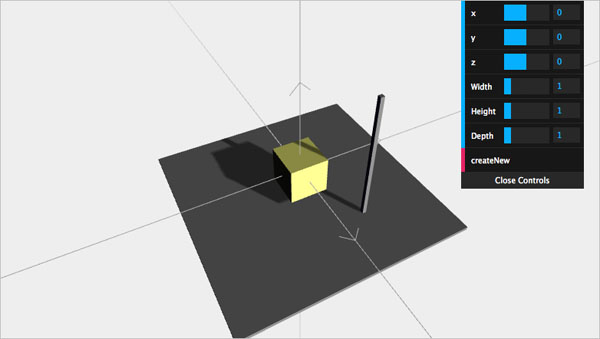
\includegraphics[scale=0.45]{images/basicsThreeJS.png}
	\caption{Three.js Example}
	\label{fig:threejs}
\end{figure}


Great examples have been created by MrDoob and by Three.js' contributors and the code is freely available. The code is relatively easy to follow and understand by even the most inexperienced Javascript developer. Hence, the code is released as Three.js' constantly growing documentation. 

Google Chrome is the recommended browser for doing and testing Three.js work. It is HTML5 compatible and slightly better than FireFox, Opera, and definitely better than IE. Additionally, Chrome’s JS engine is very fast and smooth.


Three.js' basic set up is the following. First, since we are using WebGL in this project, we create an instance of \texttt{WebGLRenderer}:

\begin{lstlisting}
var renderer = new THREE.WebGLRenderer({antialias: true});
renderer.setSize(document.body.clientWidth, document.body.clientHeight);
\end{lstlisting}

Then, we plug this render in as an HTML element. We use the \texttt{body} tag as our document container:

\begin{lstlisting}
document.body.appendChild(renderer.domElement);
\end{lstlisting}

We can also include a bit of styling to make it pretty:

\begin{lstlisting}
renderer.setClearColor( scene.fog.color, 1 );
renderer.domElement.style.position = "absolute";
renderer.domElement.style.top = MARGIN + "px";
renderer.domElement.style.left = "0px";
\end{lstlisting}

To get things better, we can create an instance of a \texttt{Scene}, add some \texttt{Fog} visual effect to it, and then add a \texttt{Cube}: 

\begin{lstlisting}
var scene = new THREE.Scene();
scene.fog = new THREE.Fog(0x050505, 2000, 4000);
scene.fog.color.setHSV(0.102, 0.9, 0.825);
var cube = new THREE.Mesh(new THREE.CubeGeometry(50, 50, 50), new THREE.MeshBasicMaterial({color: 0x000000}));
cube.position.x = 30;
cube.position.y = 40;
cube.position.z = 50;
cube.rotation.x = Math.PI / 4;
scene.add(cube);
\end{lstlisting}

The above code could be then improved by adding a \texttt{Camera} object. This camera will allow us to see the cube from different angles. Technically, all we need to do is to create a \texttt{Camera} instance, set the position and orientation of such camera, and then voila! Now we have a basic interactive world consisting of a cube in the center of the \texttt{canvas}:

\begin{lstlisting}
//PerspectiveCamera(field-of-view, viewAspectRatio, nearest, farthest);
var camera = new THREE.PerspectiveCamera(45, width / height, 1, 10000);
camera.position.z = 300;
camera.lookAt(30, 40, 50);
\end{lstlisting}

Finally, the \texttt{WebGLRenderer} renders the scene from the camera. At this point, a 3D cube will appeared in the center of the screen:

\begin{lstlisting}
renderer.render(scene, camera);
\end{lstlisting} 
  
Interested readers can find more details about Three.js at \cite{threeJS}, and about WebGL at \cite{wiki:webgl}, \cite{learningWebGL}. In the next section, We will write about the algorithms we implemented in our Web-based terrain generator.

% subsection three.js (end)
